%!TEX root = ../main.tex
\raggedbottom
\chapter{Background Study}
\label{chap:bgStudy}
This chapter presents a review of the research done on different aspects of
phishing. It starts by defining the research methodology used and continues with a further articulation of the issue at hand. To do so it views phishing from the attacker's standpoint and profiles the victim. For the remainder of it, the chapter presents the most relevant research done in the area and offers critical appraisal on the work it describes.

\section{Research methodology}
The subject and aim of the research and literature review shifted several times throughout carrying out the necessary work. However, the aim has constantly been to develop an in-depth and high-resolution image of the subject matter and base the work presented upon previous studies rather than suppositions. Throughout this dissertation, the systematic process used in doing the literature review is comprised of two procedures.

The first procedure dictates that the research should begin by firstly identifying a reputable and well established study. This paper is thoroughly read and the information relevant is extracted and processed accordingly.
The second procedure is used to deepen the understating of the subject. Based on the paper identified by procedure one, the points of interest are followed by spidering through the references. When the process of spidering brings in focus papers that are not relevant to the aim, the research should return to procedure one.

Following this method ensures that by the end of the research phase, there will be a clear and in-depth understanding of the status quo in the subject of interest. In addition, the papers included in this chapter have received a greater level of attention to produce a pertinent appraisal of the work they present.


\section{Understanding the popularity}

\subsection{Attacker's viewpoint}
In understanding why phishing attacks are so popular amongst attackers, it is
useful to view it from their perspective. A successful phishing attack circumvents most of a user's or enterprise's lines of defense. Most security
solutions are centered around detecting and preventing actions that have not
been explicitly initiated or allowed by the user. The key issue is that a
phishing attack, by definition, tricks the user into giving such information or
carrying out the actions intended by the threat actor.

Other appealing factors for the attacker are the inherent vulnerabilities and
proclivities of people. \cite{PRINCIPLES_OF_PERSUASION} has corroborated the
previous research on the subject to produce a list of principles of persuasion
used in phishing attacks. Looking at the first contact of the attacker with the
possible victim, namely the e-mail subject line, the study outlines that the
most popular means of persuasion employed by attackers are: Authority (32.24\%),
Strong affect (15.01\%) and Reciprocation (12.42\%). Given the amount of time
phishing attacks have had to organically evolve, we can be confident in saying
that these instruments gained popularity based on their positive influence on
the attack's success.

\begin{figure}[!b]
	\centering
	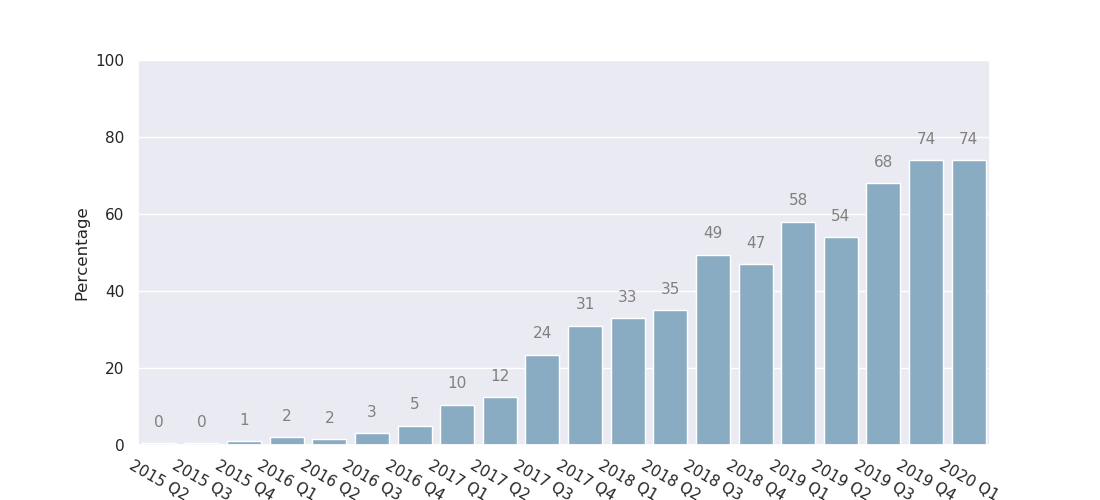
\includegraphics[width=1\textwidth]{apwg_https_usage.png}
	\caption{
		Reported number of phishing pages served over \gls{HTTPS} \citep{APWG_Q42019}}
	\label{fig:HTTPS_USAGE}
\end{figure}


\subsection{Identifying the victim}
To further the understanding of why phishing attacks are prevalent, we need to
outline the profile of the victim. A well-established study of the victim is
done by \cite{WHY_PHISHING_WORKS} which concludes the research by stating that
there is no correlation between sex, age, education, browser, operating system,
website used or hours of computer usage and the predisposition of being the victim
of a phishing e-mail. One unexpected discovery is that even in the best-case
scenarios when the subject is expecting a phishing attack, the best phishing
website deceived 90\% of the participants. The same research also describes the
elements that users look after before trusting the website, the key takeaways
being that 59\% of the participants based their decision on the page content,
with some of them (36\%) paying little attention to the address bar. The rest of
41\% based their decision on the page content and domain name, but also the
presence of \gls{HTTPS}, the padlock icon and Secure Socket Layer (\gls{SSL}) certificates.

\begin{table}[b]
	\begin{center}
		\begin{tabular}{ | m{12em} | m{12em} | m{11.5em} | }
			\hline
			                                  & \textbf{Highly susceptible} & \textbf{Less susceptible} \\
			\hline
			\textbf{Age}                      & 18-24 years old or less     & 25 years old or more      \\
			\hline

			\textbf{Gender}                   & Female                      & Male                      \\
			\hline

			\textbf{Anti-phishing training}   & No training                 & Anti-phishing trained     \\
			\hline

			\textbf{Education}                & Humanities                  & Computer science          \\
			\hline

			\textbf{Training delivery method} & Non-embedded                & Embedded                  \\
			\hline

			\textbf{Personality}              & Agreeableness               & Consciousness             \\
			\hline

			\textbf{Internet usage behaviour} & E-commerce and banking      & E-mails and browsing      \\
			\hline
		\end{tabular}
		\caption{\cite{UNDERSTANDING_PHISHING_VICTIM} on susceptibility of being a victim of phishing}
		\label{tab:VICTIM_SUSCEPTIBILITY_BREAKDOWN}
	\end{center}
\end{table}

Since this research has been done, the awareness of what \gls{HTTPS} is and it's
importance has grown substantially, but so did the number of phishing websites
served using it. The launch date of the Electronic Frontier Foundation's
\citep{EFF_LETS_ENCRYPT} certificate authority which provides \gls{SSL} certificates
at no cost can be correlated to \cite{APWG_Q42019}'s reported growing adoption
in serving phishing websites over HTTPS (Figure \ref{fig:HTTPS_USAGE}). This is
especially dangerous and confusing for the victim as \gls{HTTPS} is defined as
secure Hypertext Transport Protocol \gls{HTTP} and provides the icon of a green padlock, creating the feeling of a safe and secure website.

Other studies ventured to find correlations between personality particularities and
susceptibility of being deceived by a phishing attack, but they often are in
direct contradiction. \cite{UNDERSTANDING_PHISHING_VICTIM} managed to link the
susceptibility of being deceived by a phishing attack to a set of arbitrary
characteristics. The research concluded with the description of the two extremes
of the spectrum as shown in Table \ref{tab:VICTIM_SUSCEPTIBILITY_BREAKDOWN}.

In another study, \cite{SPEARPHISHING_IN_THE_WILD} concluded that
conscientiousness is the biggest indicator of predisposition in being deceived
by a phishing attempt. This is in direct opposition to the conclusion of
\cite{UNDERSTANDING_PHISHING_VICTIM} which identifies agreeableness as the best
indicator of high susceptibility and conscientiousness as the best indicator for
low susceptibility of being a victim.


\section{Literature Review}
There is a wealth of approaches in phishing detection and prevention presented
by the literature. To better visualize them, \cite{ML_BASED_DETECTION_FROM_URL}
sinthesised the anti-phishing detection systems' literaterature structure as shown in Figure \ref{fig:PHISHING_SOLUTION_CATEGS}. In the following subsections, the discussion will be focused on software-based, as user awareness is considered out of scope for the aim of this dissertation.

The literature review is categorized in rule-based (including black-lists, white-lists and heuristics) and machine learning-based. Some of the research does have
some hybrid aspects but has been assigned to the category deemed as most
relevant. The reason behind the selected categories lies in the fundamentally
different type of classification mechanism.

\begin{figure}[t]
	\centering
	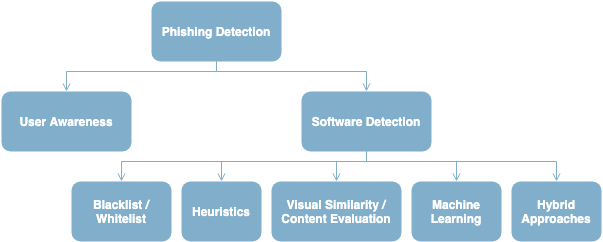
\includegraphics[width=0.9\textwidth]{phish_detection_class.png}
	\caption{
		Categorisation of phishing prevention solutions
		\citep{ML_BASED_DETECTION_FROM_URL}}
	\label{fig:PHISHING_SOLUTION_CATEGS}
\end{figure}

\subsection{Rule-based phishing detection}
\label{RULEBASED}

% (maybe speak about google safe-browsing?)

Rule-based phishing solutions classify websites as malicious or legitimate based
on a pre-defined set of rules. Because the ruleset is the centerpiece of the
detection system, the resulted performance is tightly linked it's design. As a consequence, the focus is set on rule selection and conditional relationship setting.

\cite{ANTIPHISHING_AUTOMATED_WHITELIST} proposed an automated individual
white-list capable of updating itself with records of the IP addresses of each
website visited, which features a login page. If the user attempts to submit
information through such a login user interface, they get a warning
informing them that they are doing so on a webpage outside of the white-list.
The proposed solution uses the Naive Bayesian classifier to take decisions, which
has delivered high effectiveness in previous studies on anti-spam
\citep{BAESYAN_KEYWORD_COMPARISON} and junk e-mail
\citep{BAESYAN_JUNK_FILTERING} filters. After the decision has been taken, the
classification is expected to be further confirmed by the user. Although the
proposed solution delivered a rate of true positives of 100\% and a rate of
false negatives of 0\%, the disadvantage is that this approach relies on the
involvement of the user, and cannot discover new phishing webpages.

Another white-list based approach is presented by
\cite{ANTIPHISHING_AUTOUPDATED_WHITELIST} which achieves phishing detection
using a two-phase method. In the proposed system the webpages are logically
split into "not visited" and "re-visited". The first module is triggered when a
page is re-visited and consists of a domain lookup within the whitelist. If the
domain name is found, the system matches the IP address to finally take the
decision. When the domain name is not recorded in the whitelist, the system uses
its second module. The second module is based on statistical analysis of the
number of hyperlinks pointing to a foreign domain used in a phishing webpage
compared to a legitimate one. After extraction, the system examines the features
from the hyperlinks to take the decision. Although the proposed system covers a
variety of phishing attacks (e.g. DNS poisoning, embedded objects, zero-hour
attack) it has declared experimental results of 86.02\% true positive rate and
1.48\% false-negative rate.

\cite{CANTINA} proposed an adaptation of the term frequency-inverse document
frequency (TF-IDF) information retrieval algorithm for detecting phishing
webpages in a content-based approach called CANTINA. The TF-IDF algorithm is
used to extract the most frequently used five words, which are then fed into a
search engine. The website's domain name is then compared with the top \(N\)
domain names resulted from the search, and if there is a match the website is
considered legitimate.
To lower the rate of false-positives, they included a set of heuristics checking
the age of the domain, the presence of characters such as '@' signs, dashes,
dots or IP addresses in the URL and some content-based checks such as
inconsistent well-known logos, links referenced and forms present. The
experimental results show a true positive rate of 97\% and a false positive rate
of 6\%. After the addition of these heuristics the false positive rate decreased
to 1\% but so did the true positive rate, which decreased to 89\%. An important
note about this research is that the resulted effectiveness is tightly linked to
the English language.

\cite{RULE_BASED_CLASSIFICATION} presents an intelligent rule-based phishing
detection system, whose ruleset is produced through data mining. The study
begins with a proposed list of seventeen phishing features derived from previous
work on anti-phishing detection systems. These are then fed into different
rule-based classification algorithms, each of which utilizes a different
methodology in producing knowledge. The conclusion presents C4.5 \citep{C4.5} as
the algorithm that produced the most effective ruleset. The extracted set is
comprised of features related to the request URL, age of domain, HTTPS and SSL,
website traffic, subdomain and multi subdomain, presence of prefix or suffix
separated by "--" in the domain and finally using an IP address. The downside of
the presented solution is the reliance on third-party services providing
information about the age of the domain, webpage traffic, and DNS record data.
Furthermore calibrating the thresholds for each feature requires complex
statistical work.

\begin{singlespace}
	\begin{table}[!b]
		\small
		\begin{center}
			\begin{tabular}{ m{41.5em} }
				\hline
				\\
				\(Rule\ 1: if\ \{\ Transport\ Layer\ Security\ =\ HTTP\ \cap\ Keyword\ in\ the\ path\)

				\(portion\ of\ the\ URL\ =\ yes\ \cap\ Top\ Level\ Domain\ =\ yes\ \}\ \implies\ class\ phishing\)
				\\\\
				\(Rule\ 2: if\ \{\ Number\ of\ slashes\ in\ URL\ \geq\ 5\ \cap\ Transport\ Layer\ Security\ =\ HTTP\ \cap\ Keyword\ in\ the\ path\ of\ the\ URL\ =\ yes \}\ \implies class\ phishing\)
				\\\\
				\(Rule\ 3: if\ \{\ Special\ characters\ =\ yes\ \cap\ Transport\ Layer\ Security\ =\ HTTP\ \cap\ Number\ of\ terms\ in\ the\ host\ name\ of\ the\ URL\ > 4\ \}\ \implies class\ phishing\)
				\\\\
				\(Rule\ 4: if\ \{\ Dots\ in\ the\ host\ URL\ > 4\ \cap\ Transport\ Layer\ Security\ =\ HTTP\ \cap\ Number\ of\ terms\ in\ the\ host\ name\ of\ the\ URL\ > 4\ \}\ \implies class\ phishing\)
				\\\\
				\(Rule\ 5: if\ \{\ Number\ of\ slashes\ in\ URL\ \geq 5\ \cap\ Dots\ in\ the\ host\ URL\ > 4\ \cap\ Length\ of\ the\ URL\ > 75\ \}\ \implies class\ phishing\)
				\\\\
				\(Rule\ 6: if\ \{\ Special\ characters\ =\ yes\ \cap\ Transport\ Layer\ Security\ =\ HTTP\ \cap\ Top\ Level\ Domain\ =\ yes\ \}\ \implies class\ phishing\)
				\\\\
				\(Rule\ 7: if\ \{\ Dots\ in\ the\ host\ URL\ > 4\ \cap\ Transport\ Layer\ Security\ =\ HTTP\ \cap\ Keyword\ in\ the\ path\ of\ the\ URL\ =\ yes\ \}\ \implies class\ phishing\)
				\\\\
				\(Rule\ 8: if\ \{\ Special\ characters\ =\ yes\ \cap\ Transport\ Layer\ Security\ =\ HTTP\ \cap\ Keyword\ in\ the\ path\ of\ the\ URL\ =\ yes\ \}\ \implies class\ phishing\)
				\\\\
				\(Rule\ 9: if\ \{\ Dots\ in\ the\ host\ URL\ > 4\ \cap\ Keyword\ in\ the\ path\ of\ the\ URL\ =\ yes\ \cap\ Top\ Level\ Domain\ =\ yes\ \}\ \implies class\ phishing\)
				\\\\
				\hline
			\end{tabular}
			\caption{Rule mining results of the apriori algorithm \citep{INTELLIGENT_RULE_MINING}}
			\label{tab:APRIORI_MINED_RULES}
		\end{center}
	\end{table}
\end{singlespace}

\cite{INTELLIGENT_RULE_MINING} approaches phishing detection by firstly focusing
on the extraction of key indicators that are statistically proven to be found in
phishing websites. The paper then presents a set of heuristics based on the
aforementioned statistical investigations and analysis, which are translated
into fourteen rules responsible for URL classification. Similar to
\cite{RULE_BASED_CLASSIFICATION}, the identified rules are fed into two data
mining algorithms (Apriori and Predictive Apriori), to discover effective
associations between them. The paper concluded by stating the two sets resulted
from associative rule mining, and the reported experimental accuracy of 93\%
when using the ruleset mined by the apriori algorithm. The rules used to achieve
this efficiency are presented in Table \ref{tab:APRIORI_MINED_RULES}.

\subsection{Machine-learning based phishing detection}

Machine learning-based solutions are centered around the process of feature
extraction and selection from different parts of the website such as the URL or
Hypertext Markup Language (HTML) content, and the training of a machine learning model using this
information. This subsection will briefly discuss a variety of machine learning
approaches to anti-phishing detection systems, and the key takeaways from the
studies covered.

\cite{URL_SAYS_ALL} proposes PhishDef --- a system which does on-the-fly
classification of phishing URLs based on lexical features and adaptive
regularization of weights (AROW) \citep{AROW}. The AROW algorithm offers the capability
of calibrating the classification mechanism upon making a wrong prediction. As a
result, the predictions will be of high accuracy even when the trained model is
provided with noisy data. Furthermore, PhishDef is based on an online
classification algorithm, as opposed to a batch-based one. Online classification
algorithms continuously retrain their model when encountering new data, instead
of just delivering the prediction. The accuracy of PhishDef is reported as 95\%
with an amount of noise ranging from 5\% to 10\% and above 90\% when the amount
of noise is between 10\% to 30\%. A note worth mentioning is that PhishDef
achieves the aforementioned accuracy while having low computational and memory
requirements.

Furthering the work on CANTINA mentioned in Subsection \ref{RULEBASED},
\cite{CANTINA+} enhanced the detection system by adding a feature-rich machine
learning module. The iteration is named CANTINA+, and it aims to address the
high false-positive rate of its predecessor. Besides machine learning
techniques, this enhanced iteration brings in a focus on search engines, and the
HTML Document Object Model (DOM), adding several checks on brand, domain,
hostname search and HTML attributes. Besides the inherited trade-offs of
CANTINA, the research states that one of the limitations of CANTINA+ is the
incapability of delivering predictions on phishing websites that are composed of
images, thus offering no text for it to analyze. However, while it manages to
improve upon the original implementation of CANTINA and successfully achieves an
accuracy rate of 92\%, it is still prone to producing a considerable number of
false positives.

\cite{MULTISTAGED_DETECTION_BOTNETS} presents a multi-stage detection system
that aims to both pro-actively and reactively take action against banking
bot-nets. The first feature of this model is an early warning detection module
which supervises the malicious-looking newly registered domains. The second
module does spear phishing detection using a machine learning model trained on
different variations of popular domains such as bitsquatting, omission, etc.
Although this research is geared more towards banking bot-nets, the approach
used in URL variations detection and spear-phishing protection is well designed
and highly relevant.

\cite{STACKED_ML_URL_HTML} takes a different approach by using a stacked machine
learning model that successfully surpasses the efficiency of single model
implementations of anti-phishing detection systems. The study shows the
comparison between the proposed stack composed of Gradient Boosting Decision
trees \citep{GBDT}, XGBoost \citep{XGBOOST}, and LightGBM \citep{LIGHTGBM} and
single models using algorithms such as support vector machine, nearest neighbor
classifier, decision trees, and random forest. Furthermore, it provides a wealth
of information about efficiency differences between different single or stacked
models. To measure inter-rater reliability for qualitative (categorical) items
and elect the best candidates for the stacking model \cite{STACKED_ML_URL_HTML}
used Cohen's kappa static \citep{DATA_MINING_T&T}. The resulted stack was
selected based on the aforementioned kappa static and the lower average error.
This method of selection lowered the false-positive and false-negative rates of the stacking model when compared to all its components
individually. Finally, the research reports an accuracy rate of the stacked
model of 97.3\%. with a false positive of 1.61\% and a false negative rate of
4.46\%.

\cite{ML_BASED_DETECTION_FROM_URL} researches the possibility of a real-time
anti-phishing system, training seven different classification algorithms with
natural language processing (NLP), word vector and hybrid features. In doing so,
\cite{ML_BASED_DETECTION_FROM_URL} states the lack of a worldwide acceptable
test dataset for effectiveness comparison between phishing solutions, and
proceeds to construct one containing 73,575 URLs of which 34,600 legitimate and
37,175 malicious. The paper uses this dataset to conduct comparisons between
previous work in the field and the selected classification algorithms (Decision
Trees, Adaboost, Kstar, K-Nearest Neighbour, Random Forest, Sequential Minimal
Optimization and Naive Bayes), outlining the best performers. The most effective
combination discovered is the Random Forst algorithm trained with NLP features.
It achieved an experimental accuracy of 97.98\% in URL classification, while
being language and third-party service independent, and achieving real-time
execution and detection of new websites. An important tendency emergent from the
comparisons is that the NLP features seem to improve accuracy across the
majority of machine learning algorithms covered.

\begin{center}
	\label{tab:EXISTENT_SOLUTIONS}
	\small
	\begin{tabular}{ | m{0.9em} | m{7.6em} | m{13em} | m{7.1em} | m{2.3em} | m{4.3em} | }
		\hline
		                                  & \textbf{Plugin for Phishing} & \textbf{Features \& Techniques}       & \textbf{Browser}    & \textbf{Acc \%} & \textbf{Service  type} \\
		\hline
		\multicolumn{1}{|c|}{\textbf{1}}  & GoldPhish                    & Heuristics \& Features-based          & IE                  & 98              & Free                   \\
		\hline
		\multicolumn{1}{|c|}{\textbf{2}}  & Cloudmark                    & Heuristics                            & IE                  & 94              & Free                   \\
		\hline
		\multicolumn{1}{|c|}{\textbf{3}}  & MS SmartScreen               & Blacklist and whitelist               & IE                  & 95.9            & Free                   \\
		\hline
		\multicolumn{1}{|c|}{\textbf{4}}  & Netcraft                     & Blacklist and whitelist               & Chrome, Firefox     & 90              & Free                   \\
		\hline
		\multicolumn{1}{|c|}{\textbf{5}}  & SpoofGuard                   & Heuristics \& Features-based          & IE                  & 91              & Free                   \\
		\hline
		\multicolumn{1}{|c|}{\textbf{6}}  & Phishdentity                 & Google search-by-image API            & IE                  & 97.2            & Research               \\
		\hline
		\multicolumn{1}{|c|}{\textbf{7}}  & PhishTackle                  & Heuristics \& Features-based          & IE                  & 91.3            & Research               \\
		\hline
		\multicolumn{1}{|c|}{\textbf{8}}  & PhishGuard                   & Heuristics                            & Firefox             & 94              & Research               \\
		\hline
		\multicolumn{1}{|c|}{\textbf{9}}  & PhishIdentifier              & Heuristics                            & Firefox             & 92              & Research               \\
		\hline
		\multicolumn{1}{|c|}{\textbf{10}} & PhishTester                  & Heuristics \& Features-based          & IE                  & 97.1            & Research               \\
		\hline
		\multicolumn{1}{|c|}{\textbf{11}} & CANTINA+                     & Heuristics \& Features-based          & IE                  & 98.06           & Research               \\
		\hline
		\multicolumn{1}{|c|}{\textbf{12}} & PhishAri                     & Features-based                        & Chrome              & 92.52           & Research               \\
		\hline
		\multicolumn{1}{|c|}{\textbf{13}} & PhishShield                  & Heuristics \& Feature-based           & Chrome              & 96.57           & Research               \\
		\hline
		\multicolumn{1}{|c|}{\textbf{14}} & PhishNet                     & Blacklist                             & Chrome              & 95              & Research               \\
		\hline
		\multicolumn{1}{|c|}{\textbf{15}} & PhishDef                     & Heuristics \& Feature-based           & Chrome              & 97              & Research               \\
		\hline
		\multicolumn{1}{|c|}{\textbf{16}} & GSB                          & Blacklist                             & Chrome, Firefox     & 93.3            & Free                   \\
		\hline
		\multicolumn{1}{|c|}{\textbf{17}} & PhishZoo                     & Heuristics                            & Chrome              & 96.10           & Research               \\
		\hline
		\multicolumn{1}{|c|}{\textbf{18}} & Seclayer                     & Heuristics                            & IE, Chrome          & 91              & Free                   \\
		\hline
		\multicolumn{1}{|c|}{\textbf{19}} & IPDPS                        & Heuristics \& Feature and image based & IE, Chrome, Firefox & 98.55           & Research               \\
		\hline
	\end{tabular}
	\captionsetup{type=table}\caption{A comparison of existing solutions \citep{INTELLIGENT_PHISHING_ANFIS}}
\end{center}

\cite{INTELLIGENT_PHISHING_ANFIS} studies the performance of a few machine
learning models, one of which is an artificial neural network named Adaptive
Neuro-Fuzzy Inference System \citep{ANFIS} when trained with integrated text,
image, and frame features. Before venturing to do so, the research presents a
brief comparison between the proposed solution, and numerous other anti-phishing
detection systems which can be found in Table \ref{tab:EXISTENT_SOLUTIONS}.
Throughout its content, the paper builds a set of 35 features from phishing
websites analysis and related work and compares their efficiency. These are then
bound in sets and fed into ANFIS, SVM, and KNN algorithms to study the outcome.
The ANFIS-based hybrid solution (including text, image and frame features)
delivered an accuracy of 98.30\%. Although the research considers the previously
mentioned solution as the conclusion, the ANFIS text-based classification
records an accuracy of 98.55\%. Besides this, throughout the study, there is
evidence that text-based detection systems tend to outperform image-based,
frame-based and hybrid ones.

\cite{SVM_ANTI_PHISHING} presents a solution based on a selection of seventeen
web content features which are fed into a Support Vector Machine (SVM) learning
algorithm. The most effective features are elected based on accuracy, error,
Cohen's Kappa Static \citep{DATA_MINING_T&T}, sensitivity, and the F-Measure
\citep{DATA_MINING_T&T}. Before evaluation, the features are fed into the SVM
algorithm to extract knowledge in the form of rules to increase
comprehensibility. By doing this, the importance and effect of each feature can
be extracted. The research benchmarks the features and discusses the
consequences of omitting different rules, outlining the ones with the biggest
contribution in making a correct prediction.
By using this approach the study reports an impressive experimental result of
99.14\% accuracy, with only 0.86\% false negative. Furthermore, the proposed
solution achieves zero-day phishing detection and language independence while
maintaining independence from search engines and third party services.

Finally, \cite{SVM_SIMILARITY_INDEX} focused on studying how similarity indexes
influence the accuracy of support vector machine models, the aim being the
production of a lightweight anti-phishing detection system, suitable for devices
such as smartphones. The paper first presents a set of base URL features
composed of number of hyphens, number of dots, the number of numerical
characters and IP presence. To this set \cite{SVM_SIMILARITY_INDEX} added the
classic Levenshtein distance, normalized Levenshtein distance, Jaro Winkler
distance, the longest common subsequence, Q-Gram distance, and the Hamming
distance individually, and measured the influence by comparing it to the base
accuracy. All the aforementioned additions calculate the similarity index
between two strings. This calculation is done on the entire database of two
thousand records which is incorporated in the proposed solution (1000 legitimate
URLs and 1000 malicious). The study concludes by reporting an accuracy of 95\%.
Furthermore, it states that the Hamming distance is the most effective from the
studied set, improving the overall recognition rate by 21.8\%.


\subsection{Google Safe Browsing}
Before engaging in the development of a solution meant to chanllenge the status-quo, it is of paramount importance to gain insight into what the artefact competes with. As previously stated, Google Safe Browsing is responsible for protecting the top three browsers in terms of market share: Google Chrome, Apple's Safari and Mozilla Firefox. This subsection presents work conducted to both map it's inner working as well as assess it's classification accuracy.

\begin{figure}[h]
	\centering
	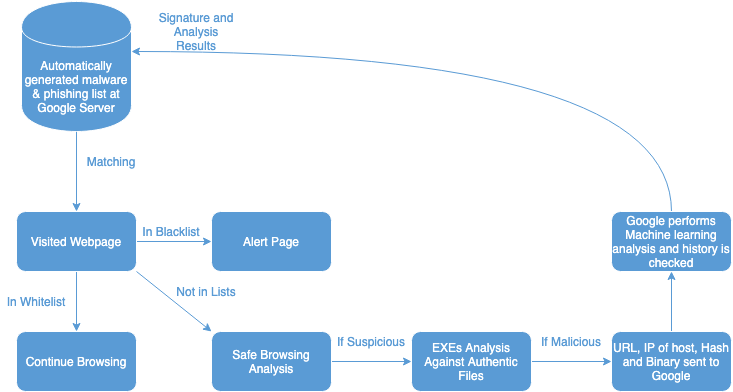
\includegraphics[width=0.95\textwidth]{google_safe_browsing.png}
	\caption{
		Architecture of Google Safe Browsing
		\citep{GOOGLE_SAFE_BROWSING_VERSIONS}}
	\label{fig:PHISHING_SOLUTION_CATEGS}
\end{figure}

\cite{GOOGLE_SAFE_BROWSING_VERSIONS} describes the mechanism behind Google Safe Browsing and captures the differences between the different API versions. However, the study dates back to 2015, so the version comparision table includes only the first three versions (Table \ref{tab:GSB_VERSIONS}). Since then, version four has been released, marking the end of support for version two and three.
\cite{GOOGLE_SAFE_BROWSING_V4} does not mention any fundamental changes to the version four API, but details a series of ajustments focusing towards the growth in usage of mobile devies. The new API is optimised around the challenges of the mobile environment: the limited power, network badwidth and poor quality of service. Furthermore, the protection per bit is maximized, due to cellular data being a direct expense of the user.

Moving to performance assessment, \cite{SECURITY_BUSTERS} presents a thorough evaluation of anti-phishing detection systems embedded in different browsers and on different platforms. In developing the proposed proof of concept security proxy, \cite{SECURITY_BUSTERS} uncovered the classification accuracy issues of popular browsers. The study compiles information on the substantial difference between phishing URL detection and malicious URL detection (Table REF). It is noticeable that from all the browsers that use GSB, Google Chrome is the better performer.

\subsection{Motivation revision}
The literaterature shows a great level of creativity in the solutions it proposes. However, the work presented in this chapter focuses on raising the bar as hight as possible regarding accuracy. Although this is a useful target to aim towards, none of them aim to improve upon existing browser protection in a manner that fits the scenario and prioritises based on the circumstances of such system.

\begin{center}
	\footnotesize
	\label{tab:OPTIMISED_MODELS}
	\begin{tabularx}{\textwidth}{ | X | X | X | }
		\hline
		                                 & \textbf{True positives} & \textbf{False negatives} \\
		\hline
		\textbf{IE (Windows)}            & 48.4\%                  & 9.9\%                    \\
		\hline
		\textbf{Opera (Windows)}         & 77.9\%                  & 8.4\%                    \\
		\hline
		\textbf{Chrome (Windows)}        & 93.0\%                  & 1.3\%                    \\
		\hline
		\textbf{Firefox (Windows)}       & 86.7\%                  & 5.9\%                    \\
		\hline
		\textbf{Opera mobile (Android)}  & 75.9\%                  & 7.9\%                    \\
		\hline
		\textbf{Firefox mobile(Android)} & 85.4\%                  & 3.4\%                    \\
		\hline
		\textbf{Safari mobile (iOS)}     & 38.7\%                  & 26.4\%                   \\
		\hline
	\end{tabularx}
	\captionsetup{type=table}\caption{Comparison of browser anti-phishing detection systems \citep{INTELLIGENT_PHISHING_ANFIS}}
\end{center}


\section{Chapter overview}
This chapter outlined the status quo of the relevant literature, expanding on
the key takeaways of each study presented. As shown, the subject of phishing is
not only prevalent in the field of security, but in psychology and others as
well. The features and mechanisms considered as most effective by the studies
presented in the rule-based and machine learning-based solutions will shape the
design of the artifact.

\begin{singlespace}
	\begin{table}[!h]
		\begin{center}
			\small
			\label{tab:GSB_VERSIONS}
			\begin{tabular}{ | m{13em} | m{12.9em} | m{13em} | }
				\hline
				\textbf{Version 1}                     &
				\textbf{Version 2}                     &
				\textbf{Version 3}                                                                                                                     \\
				\hline
				The hashing algorithm used in this
				version is MD5.                        & The hashing algorithm used in this
				version is SHA 256.                    & To improve the efficiency, protocol buffers are
				used by encoding the chunk data.                                                                                                       \\
				\hline
				The efficiency is less and it is not
				scalable.                              & In the place of a single versioned
				list, a series of "chunks” is used.    & Message Authentication Code (MAC) support
				is eliminated.                                                                        \\
				\hline
				-The entire phishing list entries are to be
				downloaded at once because the
				partial list updates are not supported
				till the time the user fully downloads
				the recent version of list.            & A list of URLs is received when the
				list of chunks is communicated
				while updating.                        & The API key format is modified. The Google
				Developers Console manages the API keys..                                                                                                      \\
				\hline
				The phishing data is given to the client in
				an order from old to new. For the
				phishing sites it is inefficient as they
				have a short lifetime.                 & The Chunks present are 32-bit
				truncated hashes                       & To differentiate between the kinds of sites and
				to allow more warnings, metadata
				functionality was used by Google-malware-
				shavar list.                                                                                                                           \\
				\hline
				As regular updates are required, so the
				bandwidth consumption is escalated.    & As soon as a match is discovered,
				the 32 bit chunk is
				communicated to Google and in
				return a list of 256 bit hash is
				acquired.                              & For the full hash, modifications are carried out
				in the cashing semantics.                                                                                                              \\
				\hline

				It is time consuming as the users scarcely
				find a match with the present pattern. & As compared to version 1, it is
				faster                                 & An expiration time is included in the HTTP
				Response for Full-Length Hashes in
				response                                                                                                                               \\
				\hline

				It is slow and has high latency.       & It has improved speed and reduced
				Latency.                               & When an update request is sent, each time the
				clients are required to wash off cashed full
				length hashes                                                                                                                          \\
				\hline
				                                       &                                                  &   Optional metadata was included in HTTP
													   Response for Full-Length Hashes                                                                                                                      \\
				\hline
				                                       &                                                  & Host keys are not used.                                                                                               \\
				\hline
			\end{tabular}

		\caption{A comparison of existing solutions \citep{INTELLIGENT_PHISHING_ANFIS}}
		\end{center}
	\end{table}
\end{singlespace}

% Background study should have between 10 and 30 papers

%[REVISIT SECTION AND GO INTO DETAIL]


% Machine learning based phishing detection from URLs
% An AI-based multi-stage detection system of banking botnets
% Intelligent web-phishing detection and protection scheme using integrated features of images, frames and text
% A comparison of Machine learning techn iques for phishing detection

%\section{Hybrid phishing detection systems}

%Hybrid phishing detection systems emerged as a natural inclination to gather the best of different categories of solutions. The strategy of combining classifiers of different nature has achieved impressive results, often surpassing the efficiency and accuracy of single category classifiers.




%A stacking model using URL and HTML features for phishing webpage detection
%GET REFERENCES FROM THE PAPER ABOVE and end with CONCLUSION

% Do an overview of research based on zero-hour protection and percentage of success





% =========================================================================================================
% Skipped compiling instructions
\iffalse
	\section{Template Text}
	Figures must be correctly numbered with captions and paragraph text should not be wrapped around figures - same rules apply to tables. An example of figures can be found below.
	\begin{figure}[t]
		\centering
		
\includegraphics[width=0.45\textwidth]{unilogo.jpg}
		\caption{Bournemouth University}
		\label{fig:BULogo2}
	\end{figure}
	You should always start with an overview (Heading 2 style) to tell what this chapter is about and finish with a summary (Heading 2 style) to tell what has been covered in this chapter.

	The Background Study (Research) or State of Art chapter is to provide your readers with information that they cannot be expected to know in detail but which they will need to know in order to fully understand and appreciate the rest of the dissertation. In short, it describes the research you have done in order to prepare for the project. You should use this section to demonstrate how much you really understand the problem domain in terms of previous (related) literature and existing solutions. For example, if your project is about developing a bespoke online CRM system for a client, this section is expected to answer the following questions:
	\begin{enumerate}
		\item What is CRM (Customer Relationship Management)?
		\item What are the characteristics of CRM?
		\item What are the main types/models of CRM?
		\item How CRM is usually implemented and what should be considered in the implementation?
		\item Are there any existing solutions and what are their advantages and limitations?
	\end{enumerate}

	\subsection{Literature Review}
	Note Literature Review is not often used as the title of this chapter even if your project is research based
\fi